\documentclass[UTF8]{article}
\usepackage{blindtext}
\usepackage[T1]{fontenc}
\usepackage[utf8]{inputenc}
\usepackage{multirow}
\usepackage{booktabs}
\usepackage{amssymb}
\usepackage{ctex}
\usepackage{tikz}
\usepackage{listings}
\usepackage[fleqn]{amsmath}
\usepackage{xcolor}
\usepackage{color}
\usepackage{xcolor}
\usepackage{graphicx}
\usepackage{epstopdf}
\definecolor{dkgreen}{rgb}{0,0.6,0}
\definecolor{gray}{rgb}{0.5,0.5,0.5}
\definecolor{mauve}{rgb}{0.58,0,0.82}
\lstset{frame=tb,
	language=C, % 使用的语言
	aboveskip=3mm,
	belowskip=3mm,
	showstringspaces=false, % 仅在字符串中允许空格
	backgroundcolor=\color{white},   % 选择代码背景,必须加上\ usepackage {color}或\ usepackage {xcolor}
	columns=flexible,
	basicstyle = \ttfamily\small,
	numbers=none, % 给代码添加行号,可取值none, left, right.
	numberstyle=\small \color{gray},  % 行号的字号和颜色
	keywordstyle=\color{blue},
	commentstyle=\color{dkgreen}, % 设置注释格式
	stringstyle=\color{mauve},
	breaklines=true,   % 设置自动断行.
	breakatwhitespace=true, % 设置是否当且仅当在空白处自动中断.
	escapeinside=``, %逃逸字符(1左面的键),用于显示中文
	frame=single, %设置边框格式
	extendedchars=false, %解决代码跨页时,章节标题,页眉等汉字不显示的问题
	xleftmargin=0em,xrightmargin=1em, aboveskip=1em, %设置边距
	tabsize=4 % 将默认tab设置为4个空格
}
\begin{document}
	\begin{center}
	\textbf{{\huge Lab4 32位MIPS流水线处理器设计}}
	\end{center}
	\section{实验目的}
	\par 
	熟悉MIPS流水线CPU的工作原理
	\section{实验过程}
	\begin{enumerate}
		\item [2.1] 学习MIP流水线处理器原理
		\par 
		通过将单周期处理器分解成5个流水线阶段来构成流水线处理器。
		
		流水线处理器在单周期处理器基础上的改变:
		\begin{enumerate}
			\item [(1)] 指令的拆分
				\par 
				单周期时一条指令直接完整执行,而流水线将单条指令拆分成5个部分,即取指令(F)、译码(D)、执行(E)、存储(M)和写回(W)。
				
				这正是流水线的实质,实现在每个阶段流水线中最多同时执行5条指令的片段。
			\item [(2)] 确保控制信号与指令保持同步
				\par
				因为在同一流水段中会执行不同指令的片段,为保证每个指令片段的控制信号与指令一致,在流水线中与特定指令相关的所有信号都必须通过流水线一起向前传播。
					
				写回阶段的寄存器文件写入逻辑在执行阶段产生,故需要对WriteReg信号做出修正,其经过存储器和写回阶段沿流水线传递,最终和ResultW一起传送到寄存器文件。
			\item [(3)] 如何解决数据冒险
				\par
				在单周期中每条指令执行完毕后再执行其他指令,因此后一条指令所需要的地址或数据已经准备好;然而流水线执行时,当一条指令试图读取前一条指令还未写回的寄存器时会发生冲突,需要在数据通路中进行冲突解决。
					
				RAW类型冲突发生的具体场景为:当前一条指令需要写寄存器且后续两条指令的任何一条读这个寄存器。
					
				同样是写寄存器,根据指令类型的不同,运用重定向或阻塞的方法来解决冲突。
					
				(1)重定向:当指令执行到E步骤时,发现所需数据与M或者W阶段的writeregM或者writeregW匹配时,可以直接使用正在传输的信号。
					
				(2)阻塞:重定向不是任何情况都适用的,如果E阶段需要使用M阶段的输出结果(如lw指令)则无法重定向。此时需要将发生冲突的指令及其后指令集体“后移”,通过重复当前阶段填充一个时间周期。
			\item [(4)] 如何解决控制冒险
				\par
				使用提前预测分支的方法,将分支前置;分支前置又会导致数据冲突,因此在解决冲突模块中也要考虑使用重定向或阻塞来解决分支前置导致的冲突。
		\end{enumerate}
		\par 以下是能处理所有冲突的流水线处理器的原理图:
		\begin{figure}[htbp]
			\centering
			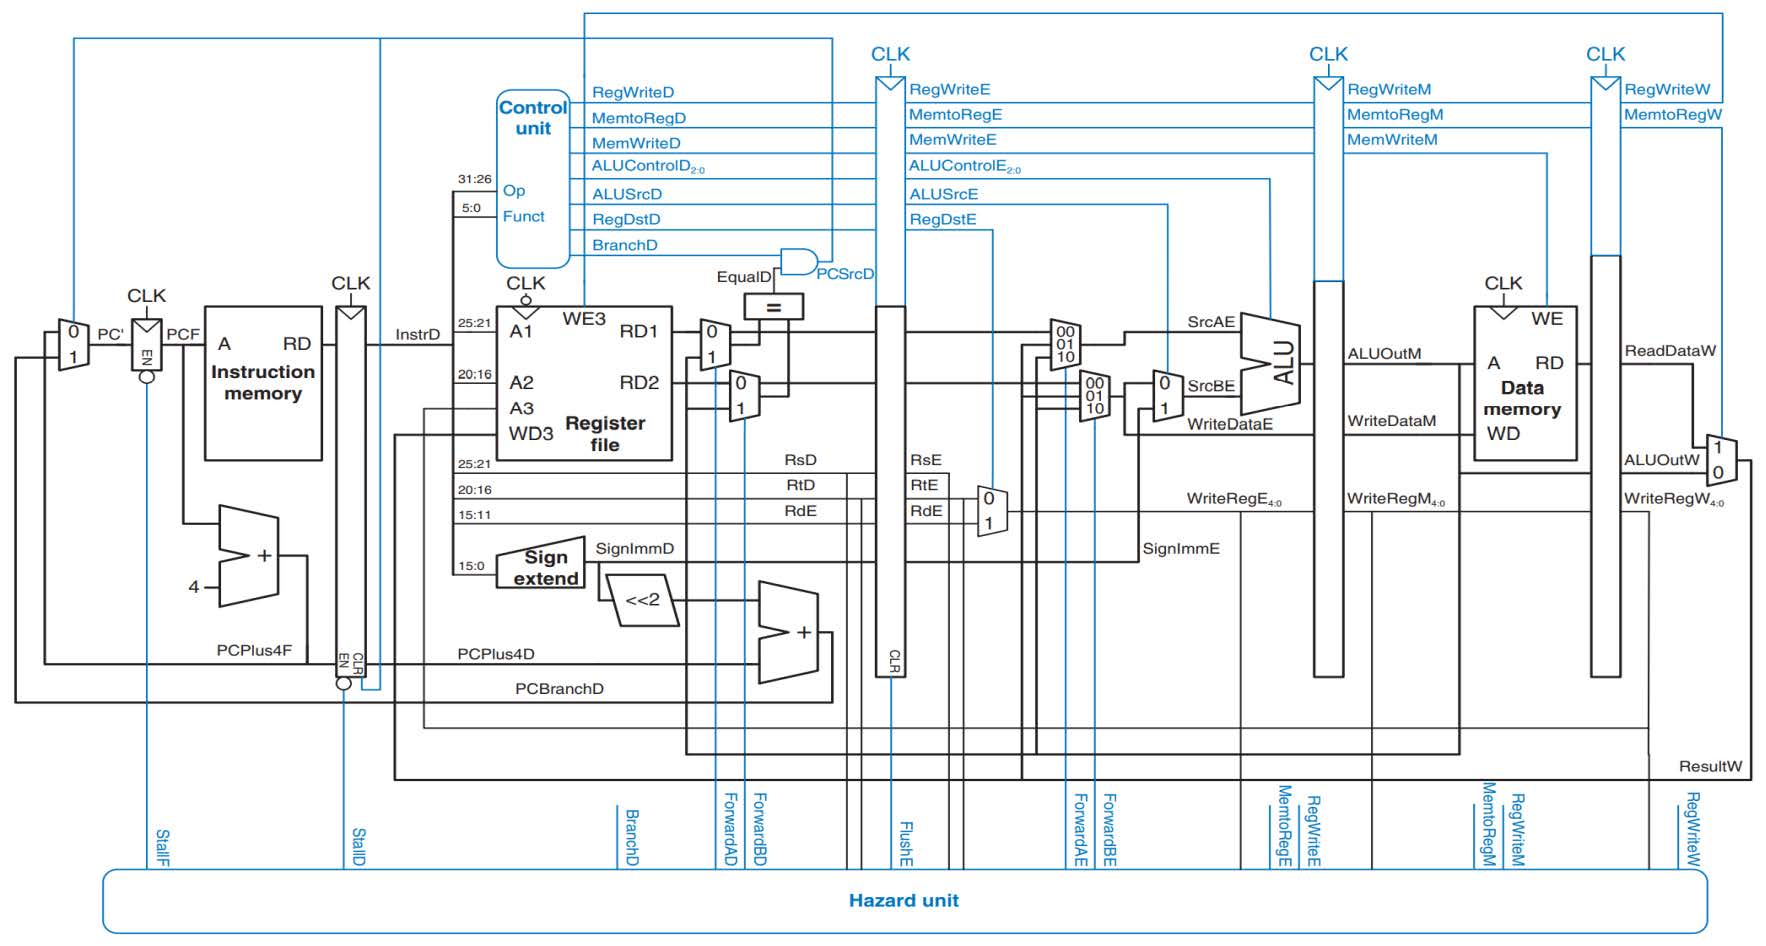
\includegraphics[scale=0.8]{2-1.jpg}
		\end{figure}
		\item [2.2] 完成MIPS流水线处理器设计
			\begin{enumerate}
				\item [2.2.1] 添加代码框架
					\par 根据上述原理,写出代码的整体结构,如下图所示:
					\begin{figure}[htbp]
						\centering
						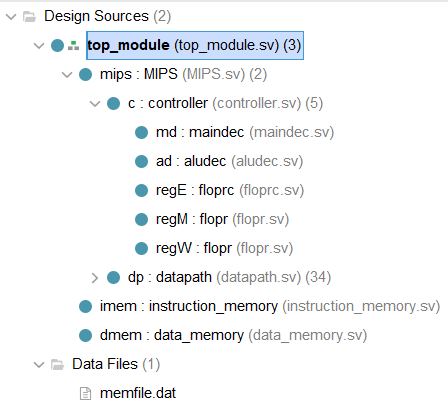
\includegraphics[scale=0.5]{2-2-1.png}
					\end{figure}
				\item [2.2.2] 基础设计
					\par 支持R类型算术/逻辑指令add、sub、and、or、slt,存储器指令lw、sw,分支指令beq
					
					数据存储器模块dmem:与单周期相同
					
					指令存储器模块imem:与单周期相同
					
					MIPS模块MIPS:
					数据通路模块datapath控制器controller:在主译码器模块maindec和ALU译码器模块aludec基础上增加流水线寄存器模块flopr和floprc,保存在流水线中与特定指令相关的所有信号,确保其通过流水线一起向前传播。
					数据通路模块datapath:划分为五个阶段,分别实例化对应模块,其中计算下一个PC在F阶段和D阶段实现,寄存器文件需要在D阶段和W阶段用到。
				\item [2.2.3] 扩展addi
					\par 增加的操作:
					
					增加零扩展元件zeroext,接受16位输入,并通过添加16个零将它们扩展到32位;
					
					增加扩展信号SorZD,当指令操作码op为andi类型时,需要进行零扩展,设置扩展SorZD为1,设置ALU操作码aluop信号为2'b11,通过ALU译码器设置ALU控制信号alucontrol为3'b000,在E阶段进行与操作;
					
					将零扩展元件zeroext的输出零扩展数据zeroImmD和符号扩展器signext的输出符号扩展数据signImmD合并到一个2输入多路复用器mux2中,为多路复用器增加 扩展信号SorZD,当这个信号为1时则立即数为零扩展,当其为0时则立即数为符号扩展;
					
					将该2输入多路复用mux2的输出扩展数据extImmD作为替代原来的符号扩展数据signImmD,传递给E阶段的signImmE,作为ALU源操作数SrcBE可选值之一。
				\item [2.2.4] 处理冒险:hazard模块
					\par 
					以下是对每种可能的冒险情况的处理方法:
					
					数据冒险:
					
					E阶段指令中一个源寄存器与M/W阶段的目标寄存器相匹配——重定向
					
					lw指令目标寄存器与D阶段源操作数相匹配——重定向
					
					分支冒险:
					
					beq指令源寄存器依赖M阶段指令ALU的结果——重定向
					
					beq指令源寄存器依赖E阶段指令ALU的结果——阻塞
					
					beq指令源寄存器依赖M阶段lw指令的结果——阻塞
			\end{enumerate}
		\item [2.3] 仿真测试
			\par 用与之间实验相同的memfile.dat进行仿真测试,结果如下图:
			\begin{figure}[htbp]
				\centering
				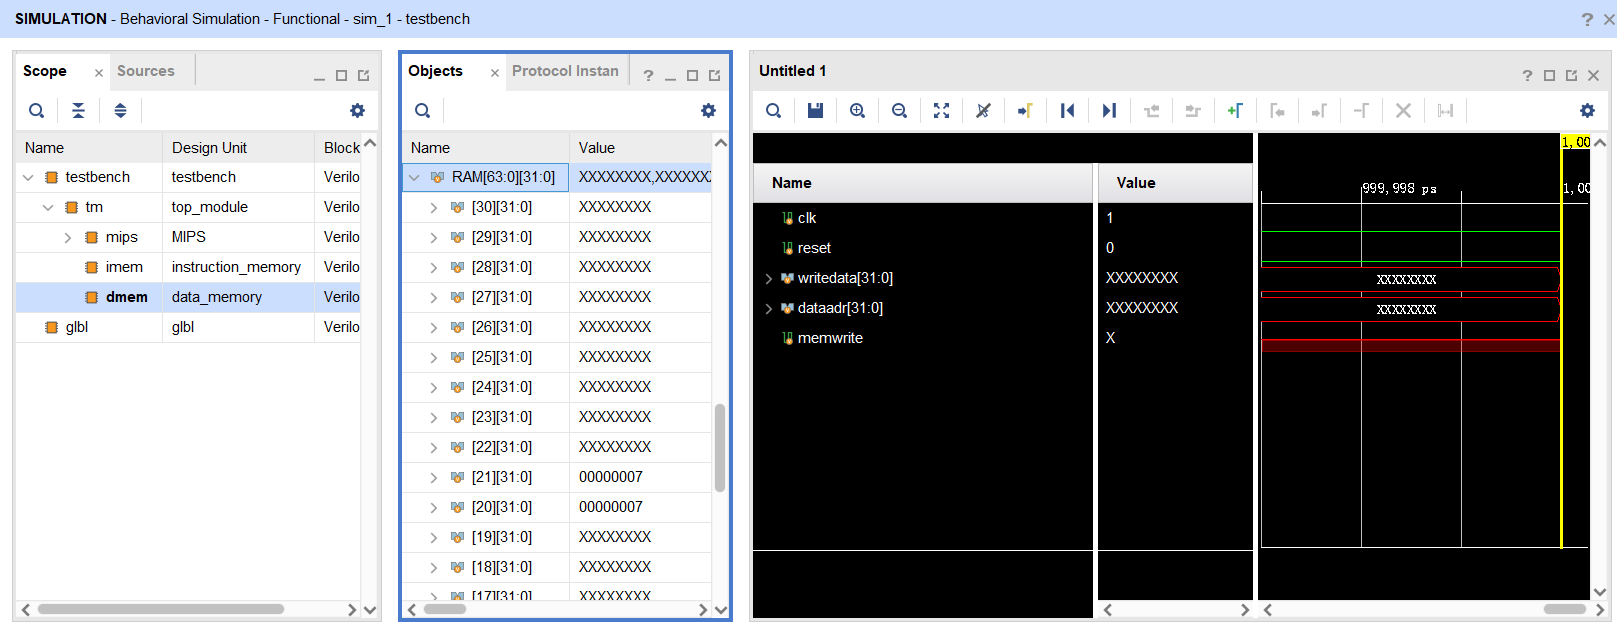
\includegraphics[scale=0.25]{2-3.png}
			\end{figure}
			\par 可以看到在内存中的21号地址(因为寻址方式与书中给出方式不同,所以地址会除以4)处存入了7,表明操作正确。
	\end{enumerate}
	\section{实现体会}
		\par 
		在本次实验中,我们成功地实现了一个32位的MIPS流水线处理器。这个过程需要精准的步骤和精妙的设计。
		
		1. 拆分指令与同步控制信号:
		我们将单周期处理器拆分成了五个阶段:取指(F)、译码(D)、执行(E)、存储(M)和写回(W)。通过这种方式,我们显著提高了处理效率。当然,为了确保每条指令在流水线中的控制信号保持同步,我们必须将这些控制信号与指令一同向前传播。
		
		2. 解决数据冒险:
		数据冒险是流水线处理器中的一个关键问题。在单周期处理中,每条指令执行完毕后再执行下一条指令,因此不会有数据冲突。但是在流水线中,当一条指令试图读取前一条指令还未写回的寄存器时,就会发生冲突。我们采用了重定向和阻塞的方法来解决这个问题。
		
		3. 解决控制冒险:
		控制冒险主要出现在分支指令中。为了减少控制冒险的影响,我们使用了提前预测分支的方法,将分支前置。这虽然解决了部分问题,但也带来了新的数据冲突。我们需要在冲突解决模块中进一步使用重定向或阻塞的方法来解决这些问题。
		
		通过这次实验,我不仅在这个过程中深刻体会到了流水线处理器的设计规范,也锻炼了自己解决复杂问题的能力。
\end{document}